%-----------------------------------------------------------------------
% 中国科学: 信息科学 中文模板, 请用 CCT-LaTeX 编译
% http://scis.scichina.com
%-----------------------------------------------------------------------

\documentclass{SCIS2020cn}
%%%%%%%%%%%%%%%%%%%%%%%%%%%%%%%%%%%%%%%%%%%%%%%%%%%%%%%
%%% 作者附加的定义
%%% 常用环境已经加载好, 不需要重复加载
%%%%%%%%%%%%%%%%%%%%%%%%%%%%%%%%%%%%%%%%%%%%%%%%%%%%%%%
\usepackage{listings}

%%%%%%%%%%%%%%%%%%%%%%%%%%%%%%%%%%%%%%%%%%%%%%%%%%%%%%%
%%% 开始
%%%%%%%%%%%%%%%%%%%%%%%%%%%%%%%%%%%%%%%%%%%%%%%%%%%%%%%
\begin{document}

%%%%%%%%%%%%%%%%%%%%%%%%%%%%%%%%%%%%%%%%%%%%%%%%%%%%%%%
%%% 作者不需要修改此处信息
\ArticleType{学生基础训练}
%\SpecialTopic{}
%\Luntan{中国科学院学部\quad 科学与技术前沿论坛}
\Year{2021}
\Vol{50}
\No{1}
\BeginPage{1}
\DOI{}
\ReceiveDate{}
\ReviseDate{}
\AcceptDate{}
\OnlineDate{}
%%%%%%%%%%%%%%%%%%%%%%%%%%%%%%%%%%%%%%%%%%%%%%%%%%%%%%%

\title{对数几率回归}{对数几率回归}

\entitle{Title}{Title for citation}

\author[1]{袁满杰}{{yuanmanjie@foxmail.com}}


\address[1]{南京大学, 南京 210023}


\AuthorMark{第一作者等}


\abstract{本文对对数几率回归理论进行了回顾,并从直接调用算法包和使用numpy从底层实现两种方法进行实践.最后在两个UCI数据集上进行了测试,并对两种方法进行了性能的比较。}


\keywords{对数几率回归, 机器学习}

\maketitle

\section{理论回顾}

对数几率回归,一般又称为逻辑回归,虽然名字中带有“回归”,但其实是一种经典的二分类算法。对数几率回归算法将二分类正负样本标记为0和1,其旨在使用线性回归,将$w^Tx+b$的结果映射到$\{0,1\}$上从而实现二分类的任务。理想情况下应使用单位阶跃函数,如\ref{eq1}所示。

\begin{equation}
    \label{eq1}
    f(x)=\begin{cases}
        0,\ \ x<0;\\
        0.5, x=0;\\
        1,\ \ x>0;
    \end{cases}
\end{equation}

然而,其具有不连续、不可导等诸多不好的数学性质,因此尝试用其它“S”形的、定义在$R$上并值域为$[0,1]$的函数。对数几率函数便是一个常用的替代函数.
\begin{equation}
    f(x)=\frac{1}{1+e^{-x}}
\end{equation}

将线性回归带入后可以得到如下式子:
\begin{equation}
    y=\frac{1}{1+e^{-w^Tx+b}}
\end{equation}

整理可得:
\begin{equation}
    \label{eq2}
    ln\frac{y}{1-y}=w^Tx+b
\end{equation}

若将$y$视为样本是正样本的可能性,则$1-y$是其为负样本的可能性,$ln\frac{y}{1-y}$也即“对数几率”。因此,以概率的形式,\ref{eq2}式可写为:
\begin{equation}
    ln\frac{p(y=1|x)}{p(y=0|x)}=w^Tx+b
\end{equation}
可解得:
\begin{equation}
    p(y=0|x)=\frac{1}{1+e^{w^Tx+b}}
\end{equation}
\begin{equation}
    p(y=1|x)=\frac{e^{w^Tx+b}}{1+e^{w^Tx+b}}
\end{equation}
用最大似然估计来估计参数$w,b$,可以写出对数似然函数如下:
\begin{equation}
    \label{loss}
    \ell (w,b)=\sum_{i=1}^m \text{ln} p(y_i|x_i;w,b)
\end{equation}
而在$y\in\{0,1\}$的二分类下,可以将$p(y_i|x_i;w,b)$做如式\ref{eq3}的重写。同时,为了简化式子,用$\hat x$表示向量$(x;1)$,用$\beta$表示参数向量$(w;b)$.
\begin{equation}
    \label{eq3}
    p(y_i|x_i;w,b)=y_i p_1(\hat x_i;\beta)+(1-y_i) p_0(\hat x_i;\beta)
\end{equation}
将式\ref{eq3}带入式\ref{loss}化简可得:
\begin{equation}
    \ell(\beta)=\sum_{i=1}^m(-y_i\beta^T\hat x_i+ln\left(1+e^{\beta^T\hat x_i}\right))
\end{equation}

使用牛顿法最小化上述损失函数,我们可以得到如下迭代公式:

\begin{equation}
    \beta^{t+1}=\beta^t-\left(\frac{\partial^2\ell(\beta)}{\partial\beta\partial\beta^T}\right)^{-1}\frac{\partial\ell(\beta)}{\partial\beta}
\end{equation}
其中一二阶导数如下:
\begin{equation}
    \frac{\partial\ell(\beta)}{\partial\beta}=-\sum_{i=1}^m\hat x_i(y_i-p_1(\hat x_i;\beta))
\end{equation}
\begin{equation}
    \frac{\partial^2\ell(\beta)}{\partial\beta\partial\beta^T}=\sum_{i=1}^m\hat x_i\hat x_i^Tp_1(\hat x_i;\beta)(1-p_1(\hat x_i;\beta))
\end{equation}

而当加入l2正则化项时,优化目标函数变为:
\begin{equation}
    \ell(\beta)=C\sum_{i=1}^m(-y_i\beta^T\hat x_i+ln\left(1+e^{\beta^T\hat x_i}\right))+\frac{1}{2}||\beta||_2^2
\end{equation}
其对应的牛顿法迭代公式中的偏导数项变为:
\begin{equation}
    \label{eq11}
    \frac{\partial\ell(\beta)}{\partial\beta}=-C\sum_{i=1}^m\hat x_i(y_i-p_1(\hat x_i;\beta))+\beta
\end{equation}
\begin{equation}
    \label{eq12}
    \frac{\partial^2\ell(\beta)}{\partial\beta\partial\beta^T}=C\sum_{i=1}^m\hat x_i\hat x_i^Tp_1(\hat x_i;\beta)(1-p_1(\hat x_i;\beta))+I
\end{equation}
其中$I$为单位矩阵。

\section{数据集选取 }
因为对数几率回归算法是针对二分类的算法,因此选取了2个无缺失数据的二分类数据集,其中第一个数据集为对识别癌症的数据集,维度较少,难度容易。第二个数据集为根据语音特征识别帕金森病的数据集,维度较高,难度也较大。具体数据集的信息参见表\ref{tb1}

\begin{table}[!t]
    \cnentablecaption{各数据集信息表}{}
    \label{tb1}
    \begin{center}
        \begin{tabular}{@{}cccc@{}}
            \toprule
            数据集                 & 样本数 & 特征数 & 正负样本比 \\ \midrule
            WDBC                & 569 & 31  & 1.68  \\
            Parkinson's Disease & 756 & 754 & 2.93  \\ \bottomrule
        \end{tabular}
    \end{center}
\end{table}

训练时以固定随机数种子随机以8:2切分训练集和测试集。

\section{算法包调用 }

算法包使用sklearn库的LogisticRegression实现。参数上采用默认参数,即使用l2正则化且正则化参数为1.对于两个数据集的实验结果如表\ref{tb2}所示。

\begin{table}[]
    \cnentablecaption{算法包调用结果表}{}
    \label{tb2}
    \begin{center}
        \begin{tabular}{@{}ccccc@{}}
            \toprule
            数据集                 & Accuracy & Precision & Recall & F1-score \\ \midrule
            WDBC                & 0.93     & 0.93      & 0.93   & 0.93     \\
            Parkinson's Disease & 0.75     & 0.74      & 0.58   & 0.57     \\ \bottomrule
            \end{tabular}
    \end{center}
    \end{table}

\section{自己实现}
\subsection{实现过程}
自己实现基于\ref{eq11}和\ref{eq12}两式的牛顿法迭代公式,并做出了部分细节上修改:

\begin{enumerate}
    \item Hessian矩阵可能奇异、不可逆:使用了伪逆代替;
    \item 计算Sigmoid时幂运算容易数据过大出现上溢:对幂运算后的数据进行了截断,使运算结果在$[0,10^{14}]$之间;
    \item 权重初始化不合适,导致特征维数多的数据的全部样本在计算Sigmoid时易出现上溢,大量丢失计算精度,进而出现不收敛等现象:首先对数据做归一化处理,其次权重初始化为$\frac{1}{m}$,其中$m$为特征维数;
\end{enumerate}

\subsection{实现结果}
自己手动实现的结果如表\ref{tb3}所示。
\begin{table}[]
    \cnentablecaption{自己实现结果表}{}
    \label{tb3}
    \begin{center}
        \begin{tabular}{@{}ccccc@{}}
            \toprule
            数据集                 & Accuracy & Precision & Recall & F1-score \\ \midrule
            WDBC                & 0.97     & 0.98      & 0.97   & 0.97     \\
            Parkinson's Disease & 0.84     & 0.83      & 0.76   & 0.79     \\ \bottomrule
            \end{tabular}
    \end{center}
\end{table}

可以看到,或许是采用了归一化、更合适的参数初始化的原因,自己实现的对数几率回归算法在表现上比调用sklearn库中的效果更好,尤其对于高维的数据集上表现有十分明显的提升。

%%%%%%%%%%%%%%%%%%%%%%%%%%%%%%%%%%%%%%%%%%%%%%%%%%%%%%%
%%% 致谢
%%% 非必选
%%%%%%%%%%%%%%%%%%%%%%%%%%%%%%%%%%%%%%%%%%%%%%%%%%%%%%%
%\Acknowledgements{致谢.}

%%%%%%%%%%%%%%%%%%%%%%%%%%%%%%%%%%%%%%%%%%%%%%%%%%%%%%%
%%% 补充材料说明
%%% 非必选
%%%%%%%%%%%%%%%%%%%%%%%%%%%%%%%%%%%%%%%%%%%%%%%%%%%%%%%
%\Supplements{补充材料.}

%%%%%%%%%%%%%%%%%%%%%%%%%%%%%%%%%%%%%%%%%%%%%%%%%%%%%%%
%%% 参考文献, {}为引用的标签, 数字/字母均可
%%% 文中上标引用: \upcite{1,2}
%%% 文中正常引用: \cite{1,2}
%%%%%%%%%%%%%%%%%%%%%%%%%%%%%%%%%%%%%%%%%%%%%%%%%%%%%%%
\begin{thebibliography}{99}

\bibitem{1} 周志华. "机器学习 (北京: 清华大学出版社) Zhou ZH 2016." Machine Learning (2016).

\bibitem{2} Pedregosa, Fabian, et al. "Scikit-learn: Machine learning in Python." the Journal of machine Learning research 12 (2011): 2825-2830.

\bibitem{3} 手写逻辑回归(带l2正则). https://zhuanlan.zhihu.com/p/81419198


\end{thebibliography}

\end{document}
%%%%%%%%%%%%%%%%%%%%%%%%%%%%%%%%%%%%%%%%%%%%%%%%%%%%%%%
%%% 附录章节, 自动从A编号, 以\section开始一节
%%% 非必选
%%%%%%%%%%%%%%%%%%%%%%%%%%%%%%%%%%%%%%%%%%%%%%%%%%%%%%%
%\begin{appendix}
%\section{附录}
%附录从这里开始.
%\begin{figure}[H]
%\centering
%%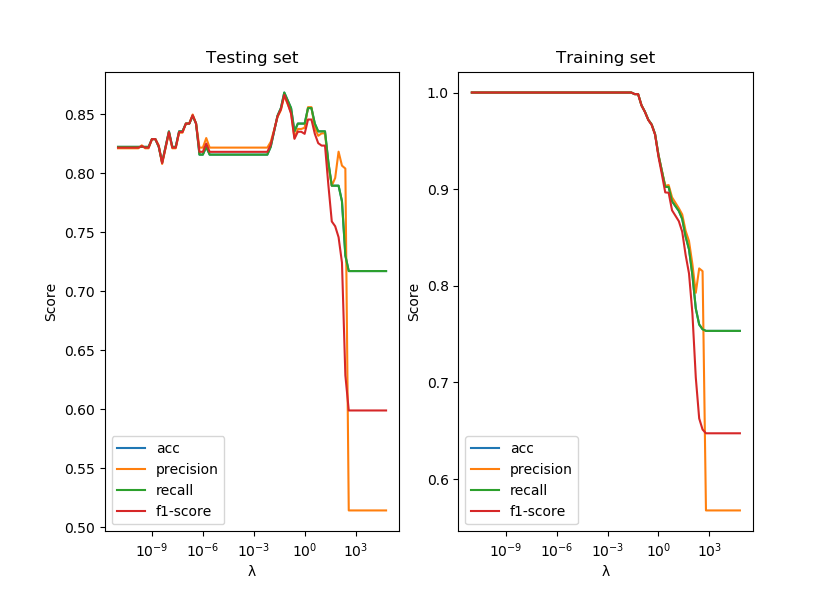
\includegraphics{fig1.eps}
%\cnenfigcaption{附录里的图}{Caption}
%\label{fig1}
%\end{figure}
%\end{appendix}